\subsection{Signaling and Call Session Management}

The signaling and call session management subsystem is responsible for establishing, maintaining, and terminating communication sessions between users. Unlike the media transmission subsystem, signaling does not carry voice data. Instead, it coordinates call setup procedures, user discovery, session negotiation, and call control operations.

This subsystem ensures that both participants are available, authenticated, and prepared before real-time voice transmission begins.

\vspace{0.5cm}
\begin{figure}[H]
    \centering
    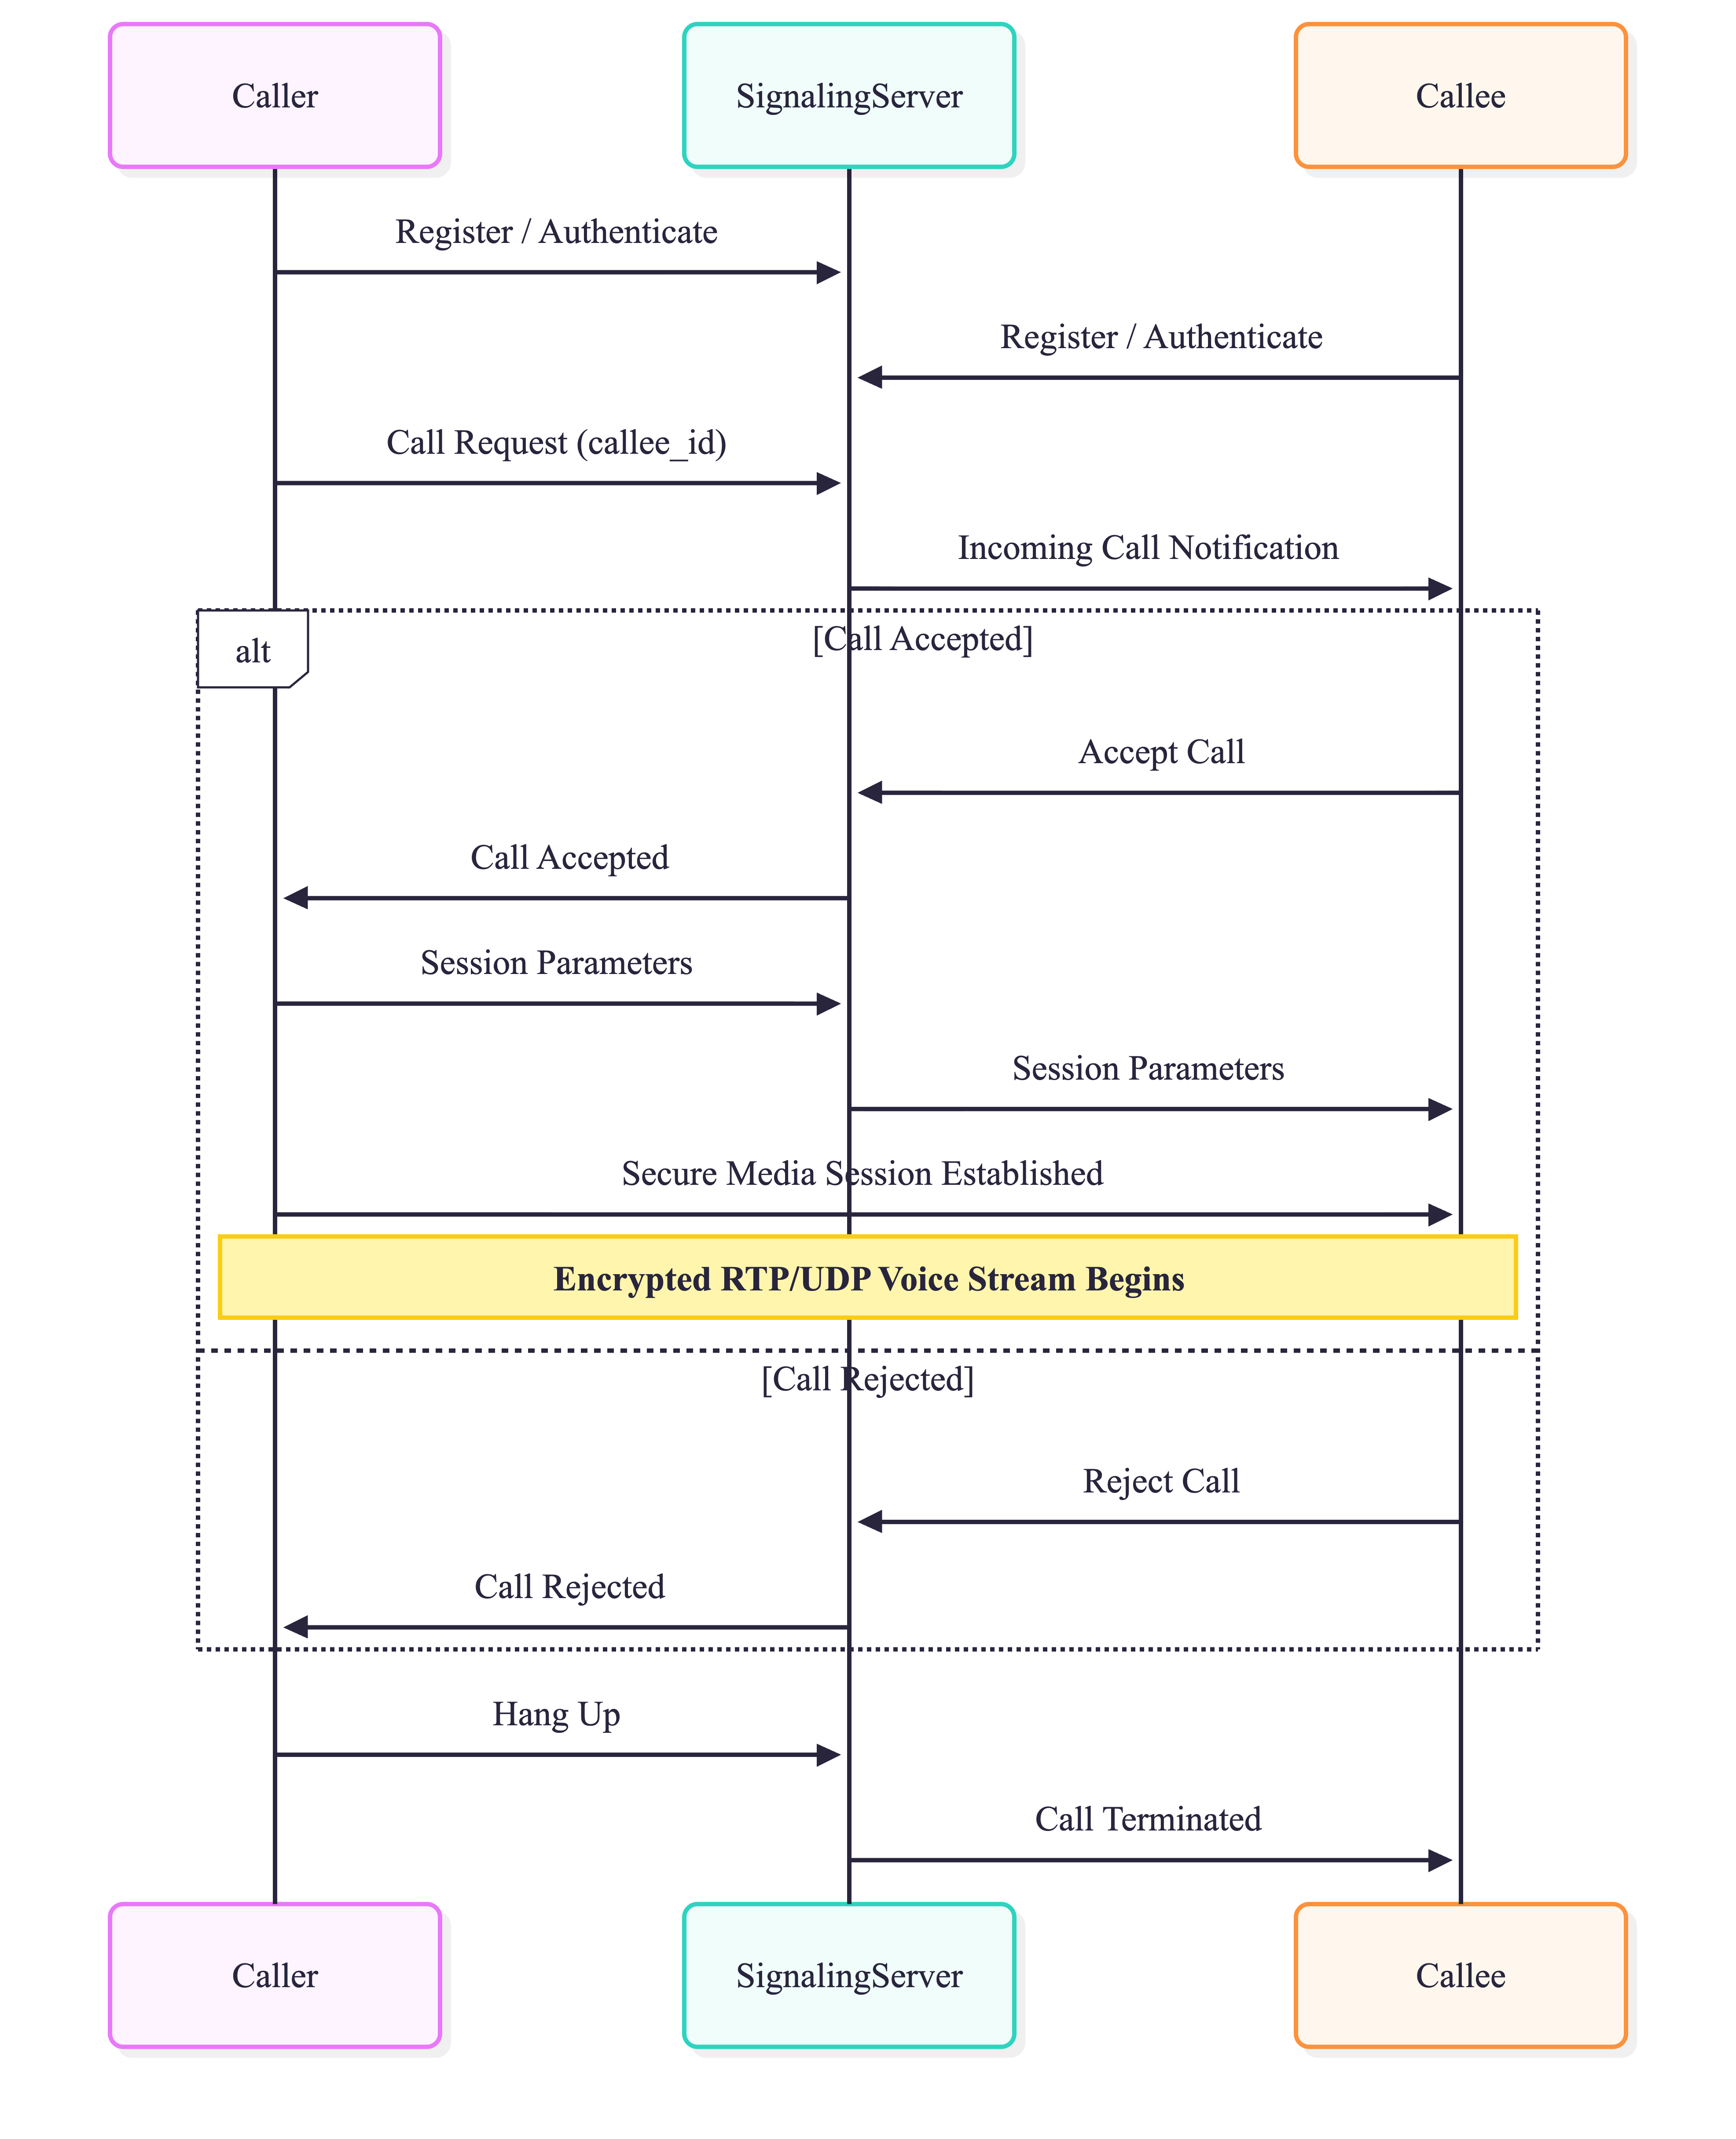
\includegraphics[width=1\textwidth]{images/methodology/call_session.png}
    \caption{Signaling and Call Session Management Sequence}
    \label{fig:call_session}
\end{figure}

\subsubsection{User Registration and Presence Management}

Before initiating or receiving calls, users must register with the signaling server. During registration, user identity information and connection details are associated with an active session.

The signaling server maintains user presence information, allowing the system to determine whether a user is online, offline, or currently engaged in another call.

This information enables efficient call routing and availability checking.

\subsubsection{Call Initiation}

When a user initiates a call, the client application sends a call request to the signaling server containing the intended recipient's identifier.

The signaling server validates the request, verifies the recipient's availability, and forwards an incoming call notification to the destination user.

At this stage, no voice packets are transmitted. The system is solely responsible for establishing communication intent between the participating users.

\subsubsection{Call Acceptance and Rejection}

Upon receiving an incoming call notification, the recipient may either accept or reject the call.

If the call is rejected, the signaling server notifies the caller and the session establishment process is terminated.

If the call is accepted, both parties proceed to session establishment and communication parameter exchange.

\subsubsection{Session Establishment}

Following call acceptance, the signaling subsystem facilitates the exchange of session-related information required for voice communication.

This information includes network endpoints, encryption parameters, session identifiers, and other metadata necessary for secure communication.

Once both participants have successfully exchanged and validated the required information, a communication session is established.

\subsubsection{Call Maintenance}

Throughout the duration of the call, the signaling subsystem remains responsible for managing session state and control messages.

Typical operations include participant status monitoring, connection supervision, call hold requests, and network state updates.

These control functions ensure that the communication session remains synchronized between participants.

\subsubsection{Call Termination}

A call session may be terminated by either participant. When a termination request is issued, the signaling server informs the remote participant and updates the session state accordingly.

Upon termination, all communication resources, temporary session information, and active media channels associated with the call are released.

This process ensures proper cleanup and prepares the system for future communication sessions.

\subsubsection{Relationship with Media Transmission}

The signaling subsystem is responsible only for call control and session coordination. Once a call session has been successfully established, real-time voice communication is performed by the media transmission subsystem.

As a result, the signaling server manages the call lifecycle while the sender-side, network transmission, and receiver-side components handle the actual voice data exchange.
